% Grossmont College -- Chem 141 Lab 5: Analysis of a Two-Component Alloy
% Cameron Carroll
% March 2014


\documentclass[fleqn,titlepage]{article}

\renewcommand*\rmdefault{ppl}

\usepackage[version=3]{mhchem} % Package for chemical equation typesetting
\usepackage{tabu}
\usepackage{wasysym}
\usepackage{listings}
\usepackage{scrextend}
\lstset{language=Matlab}
\usepackage{multirow}

% set 1" margins on 8.5" x 11" paper
% top left is measured from 1", 1"
\topmargin 0in
\oddsidemargin 0in
\evensidemargin 0in
\headheight 0in
\headsep 0in
\topskip 0in
\textheight 9in
\textwidth 6.5in

\usepackage{graphicx} % Required for the inclusion of images

\setlength\parindent{0pt} % Removes all indentation from paragraphs

\renewcommand{\labelenumi}{\alph{enumi}.} % Make numbering in the enumerate environment by letter rather than number (e.g. section 6)

%\usepackage{times} % Uncomment to use the Times New Roman font

%----------------------------------------------------------------------------------------
% DOCUMENT INFORMATION
%----------------------------------------------------------------------------------------

\begin{document}

\begin{titlepage}
  \mbox{}\\[1.25cm]
  \textbf{\LARGE Cameron Carroll \\ Grossmont College}\\[2.25cm]
  \begin{center}
    \textbf{\huge Lab 5: \\ Analysis of a Two-Component Alloy}\\[2.50cm]
  \end{center}
  \textbf{\LARGE Professor: Martin Larter \\ Chemistry 141-0692} \\
  \vfill
  \center{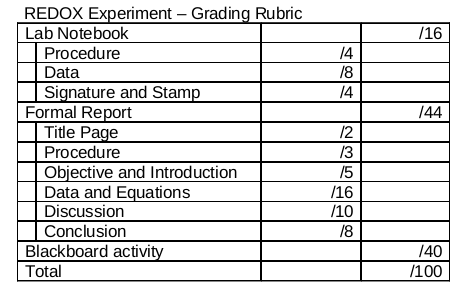
\includegraphics{./rubic_redox}}
  \center{\textbf{\LARGE Performed --} {\LARGE March 6 \& 11, 2014}}
  \center{\textbf{\LARGE Submitted --} {\LARGE March 20, 2014}}
\end{titlepage}

%----------------------------------------------------------------------------------------
% SECTION 1
%----------------------------------------------------------------------------------------
\section*{Procedure}
\begin{itemize}
  \item  \textbf{Referenced From:} \\
    \begin{addmargin}[1em]{1em}
      Lehman, J. (Et al), `Analysis of a Two-Component Alloy' \\
      Grossmont College, Chemistry 141 Lab Manual, 6th edition, pp 67-72 \\
      El Cajon, California
    \end{addmargin}
\end{itemize}

%----------------------------------------------------------------------------------------
% SECTION 3
%----------------------------------------------------------------------------------------
\section*{Data Summary \& Calculations}
  \paragraph{} (See next, handwritten, pages.)

%----------------------------------------------------------------------------------------
% SECTION 4
%----------------------------------------------------------------------------------------
\newpage
\section*{Discussion}
\paragraph{} I believe my data is okay: Not spectacularly precise but representative of the alloy. My percents by mass were 57.51 and 56.3... compared to a true value of 58.67\% Zn, this gives a 1.98 and 4.06\% error respectively. Some of this error is probably from leaks: The apparatus and tubing was certainly not perfect and some gas might have escaped while capping the reaction flask. The temperatures were probably not very accurate either because the difficulty in taking readings from the vapor and water meant a few seconds of time with lab air mixing into the system. Also, I forgot to take the barometric pressure reading for both lab sessions, and had to duplicate the value over to the other trial. Finally, I might have been too focused on blowing up the hydrogen gas -- I should have just saved my efforts for the finale.
\paragraph{} The values for alloy composition are 2\% away, which is a pretty big gap. I attribute this partially to that incorrect barometric pressure value, but poor measurements are just as likely.

%----------------------------------------------------------------------------------------
% SECTION 5
%----------------------------------------------------------------------------------------
\section*{Conclusion}
\paragraph{} Experimentally, my alloy was 56.9\% Zn and 43.10\% Al (averaged percent by mass.) The true values were 58.67\% Zn and 41.33\% Al.


\end{document}